\documentclass[tikz,border=20pt]{standalone}
\usetikzlibrary{calc}

\begin{document}
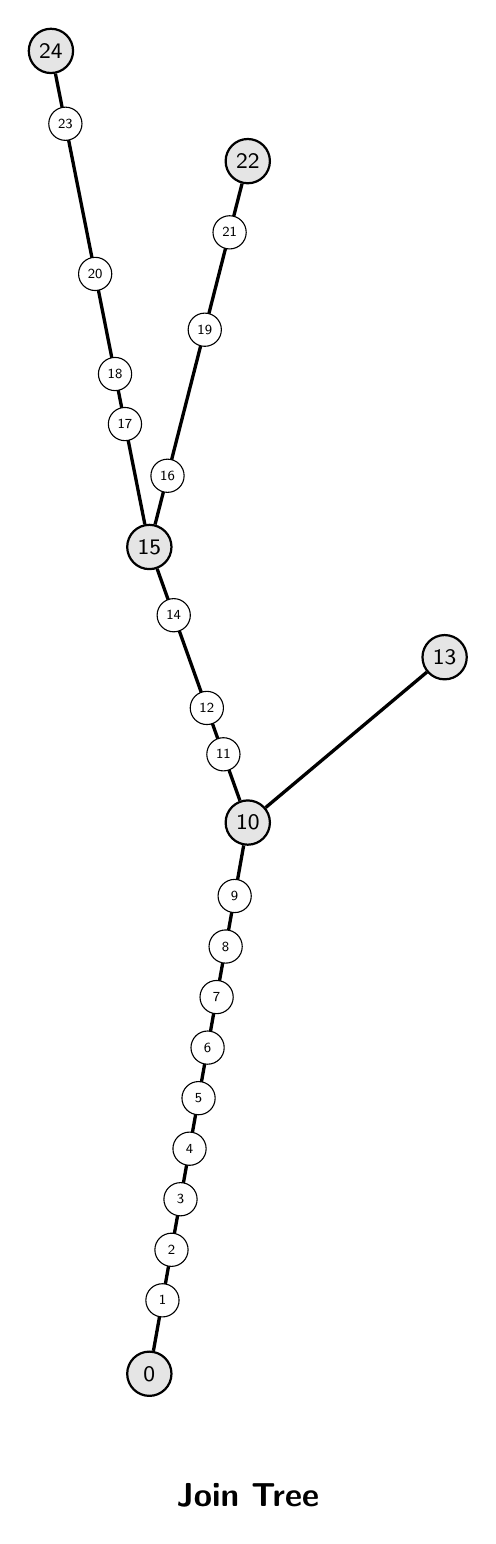
\begin{tikzpicture}[
    y=0.7cm, x=2.5cm,
    crit node/.style={circle, draw=black, fill=gray!20, thick, inner sep=1pt, minimum size=16pt, font=\sffamily\footnotesize},
    reg node/.style={circle, draw=black, fill=white, inner sep=0.5pt, minimum size=12pt, font=\sffamily\tiny},
    main edge/.style={very thick, draw=black}
]

% 关键点 (极大值与鞍点)
\node[crit node] (J24) at (0, 24) {24};
\node[crit node] (J22) at (1, 22) {22};
\node[crit node] (J15) at (0.5, 15) {15};
\node[crit node] (J13) at (2, 13) {13};
\node[crit node] (J10) at (1, 10) {10};
\node[crit node] (J0)  at (0.5, 0) {0};

% 连线与普通节点填充
\draw[main edge] (J15) -- (J24);
\foreach \v in {17, 18, 20, 23} \path (J15) -- (J24) node[pos={(\v-15)/(24-15)}, reg node] {\v};

\draw[main edge] (J15) -- (J22);
\foreach \v in {16, 19, 21} \path (J15) -- (J22) node[pos={(\v-15)/(22-15)}, reg node] {\v};

\draw[main edge] (J10) -- (J15);
\foreach \v in {11, 12, 14} \path (J10) -- (J15) node[pos={(\v-10)/(15-10)}, reg node] {\v};

\draw[main edge] (J10) -- (J13); 

\draw[main edge] (J0) -- (J10);
\foreach \v in {1, 2, 3, 4, 5, 6, 7, 8, 9} \path (J0) -- (J10) node[pos={(\v-0)/(10-0)}, reg node] {\v};

\node[font=\sffamily\bfseries\large] at (1, -2.2) {Join Tree};

\end{tikzpicture}
\end{document}
